%%
%% This is file `mcmthesis-demo.tex',
%% generated with the docstrip utility.
%%
%% The original source files were:
%%
%% mcmthesis.dtx  (with options: `demo')
%% !Mode:: "TeX:UTF-8"
%% -----------------------------------
%%
%% This is a generated file.
%%
%% Copyright (C)
%%     2010 -- 2015 by latexstudio
%%     2014 -- 2016 by Liam Huang
%%
%% This work may be distributed and/or modified under the
%% conditions of the LaTeX Project Public License, either version 1.3
%% of this license or (at your option) any later version.
%% The latest version of this license is in
%%   http://www.latex-project.org/lppl.txt
%% and version 1.3 or later is part of all distributions of LaTeX
%% version 2005/12/01 or later.
%%
%% This work has the LPPL maintenance status `maintained'.
%%
%% The Current Maintainer of this work is Liam Huang.
%%
\documentclass{mcmthesis}
\mcmsetup{CTeX = true,   % 使用 CTeX 套装时,设置为 true
        tcn = 57868, problem = A,
        sheet = true, titleinsheet = true, keywordsinsheet = true,
        titlepage = true, abstract = true}
\usepackage{palatino}
\usepackage{caption}
\usepackage{amsmath}
\usepackage{lipsum}
\usepackage{times}
\usepackage{mathptmx}

\title{Managing The Zambezi River}
\author{Kai Feng, Song Lu, Yutao Zeng}
\date{\today}
\begin{document}
\begin{abstract}
Here is the abstract to be written!
\begin{keywords}
keyword1; keyword2
\end{keywords}
\end{abstract}
\maketitle
\section{Introduction}
The Kariba Dam is one of the biggest dam in the world, which is constructed on the Zambezi River. It supplies 1626 megawatts of electricty to parts of both Zambia and Zimbabwe and \\
\lipsum[2]
\begin{itemize}
\item minimizes the discomfort to the hands, or
\item maximizes the outgoing velocity of the ball.
\end{itemize}
We focus exclusively on the second definition.

\begin{itemize}
\item the initial velocity and rotation of the ball,
\item the initial velocity and rotation of the bat,
\item the relative position and orientation of the bat and ball, and
\item the force over time that the hitter hands applies on the handle.
\end{itemize}
\lipsum[3]
\begin{itemize}
\item the angular velocity of the bat,
\item the velocity of the ball, and
\item the position of impact along the bat.
\end{itemize}
\lipsum[4]
\emph{center of percussion} [Brody 1986], \lipsum[5]

\begin{Theorem} \label{thm:latex}
\LaTeX
\end{Theorem}
\begin{Lemma} \label{thm:tex}
\TeX .
\end{Lemma}
\begin{proof}
The proof of theorem.
\end{proof}

\subsection{Other Assumptions}
\lipsum[6]
\begin{itemize}
\item
\item
\item
\item
\end{itemize}

\lipsum[7]

\section{Analysis of the Problem}
\begin{figure}[h]
\small
\centering
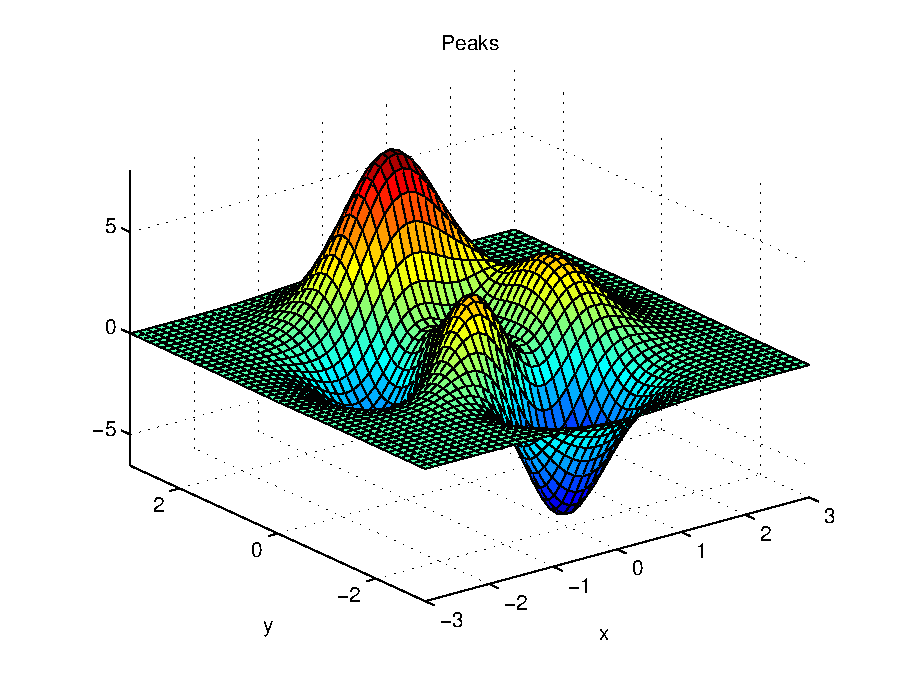
\includegraphics[width=12cm]{mcmthesis-aaa.eps}
\caption{aa} \label{fig:aa}
\end{figure}

\lipsum[8] \eqref{aa}
\begin{equation}
a^2 \label{aa}
\end{equation}

\[
  \begin{pmatrix}{*{20}c}
  {a_{11} } & {a_{12} } & {a_{13} }  \\
  {a_{21} } & {a_{22} } & {a_{23} }  \\
  {a_{31} } & {a_{32} } & {a_{33} }  \\
  \end{pmatrix}
  = \frac{{Opposite}}{{Hypotenuse}}\cos ^{ - 1} \theta \arcsin \theta
\]
\lipsum[9]

\[
  p_{j}=\begin{cases} 0,&\text{if $j$ is odd}\\
  r!\,(-1)^{j/2},&\text{if $j$ is even}
  \end{cases}
\]

\lipsum[10]

\[
  \arcsin \theta  =
  \mathop{{\int\!\!\!\!\!\int\!\!\!\!\!\int}\mkern-31.2mu
  \bigodot}\limits_\varphi
  {\mathop {\lim }\limits_{x \to \infty } \frac{{n!}}{{r!\left( {n - r}
  \right)!}}} \eqno (1)
\]

\section{Calculating and Simplifying the Model  }
\lipsum[11]

\section{The Model Results}
\lipsum[6]

\section{Validating the Model}
\lipsum[9]

\section{Conclusions}
\lipsum[6]

\section{A Summary}
\lipsum[6]

\section{Evaluate of the Mode}

\section{Strengths and weaknesses}
\lipsum[12]

\subsection{Strengths}
\begin{itemize}
\item \textbf{Applies widely}\\
This  system can be used for many types of airplanes, and it also
solves the interference during  the procedure of the boarding
airplane,as described above we can get to the  optimization
boarding time.We also know that all the service is automate.
\item \textbf{Improve the quality of the airport service}\\
Balancing the cost of the cost and the benefit, it will bring in
more convenient  for airport and passengers.It also saves many
human resources for the airline. \item \textbf{}
\end{itemize}

\begin{thebibliography}{99}
\bibitem{1} D.~E. KNUTH   The \TeX{}book  the American
Mathematical Society and Addison-Wesley
Publishing Company , 1984-1986.
\bibitem{2}Lamport, Leslie,  \LaTeX{}: `` A Document Preparation System '',
Addison-Wesley Publishing Company, 1986.
\bibitem{3}\url{http://www.latexstudio.net/}
\bibitem{4}\url{http://www.chinatex.org/}
\end{thebibliography}

\clearpage
\section{Brief Assessment of the options}
\indent \indent The solution to the Kariba Dam problem can simply be divided into three options: repairing it, rebuilding it or removing it then replacing it with other dams. To the third method, ZRA suggests to build $10\sim20$ small dams to replace the huge Kariba Dam.\\
\indent Evaluating the options from the perspective of cost and benefit is a complex task, since it can be influence by a number of factors. Only considering the cost of building dams, although it can be estimated accurately by using the cost formula below \\
\[
C_{p} = K\left(\frac{V}{\left(\frac{H}{0.3}\right)^{0.3}}\right)^{0.82}
\]
where $C_{p}$ is the cost of building the hydropower station, $V$ is the installed capacity, $H$ is the design head, $K$ is the proportional coefficient. However, the ecological costs of dam construction need to be considered more cautiously because damage to the ecological environment may be irreversible.\\
\indent Option 1. Repairing the existing Kariba Dam. This is the option with the lowest cost of construction. Meanwhile, it won't change the submerged area, so there is no extra ecological cost. From the aspect of revenue, the reconstruction and expansion of Kariba Dam hydropower station can be carried out at the same time, which can effectively increase the total installed capacity of hydropower station, and thus improve the income of hydropower station. In fact, the expansion of the Kariba Dam hydropower station is underway. Since the reconstruction will not affect the Kariba Lake, the benefits from the use of water from the lake won't be reduced. The analysis above is based on the assumption that the climate will not change drastically in the future and no rare disasters which is outside the historical statistics will occur.\\
\indent Option 2. Rebuilding the existing Kariba Dam. Because rebuilding the Kariba Dam need to remove the existing the dam and rebuild it at the origin site, it is an option with high risk and cost. What's more, the reconstruction of the dam will inevitably lead to the result that the hydropower station can't generate electricity in quite a long period, so this part of loss should also be included in the cost of reconstruction. However, rebuilding dams do have benefits. It helps to expand the installed capacity of hydropower station (benefit from re-designing the internal structure and using more advanced equipment). The new designed Dam would have better flood protection capacity, which allows river management to handle emergency with more flexibility. Stronger water storage capacity means we can raise the water level of Kariba Lake. It will increase the energy generation as well as bring the risk of ecologic damage which needs to be treated with caution.\\
\indent Option 3. Removing the Kariba Dam and replacing it with a series of $10\sim20$ smaller dams along the Zambezi River. This is quite an ambitious plan. Even if the sum of installed capacity of all these small dams is the same as that of Kariba Dam, the total construction cost is still expected to be higher than rebuilding Kariba Dam according to the cost formula above. With the same problem as option 2, removing Kariba Dam will definitely lead to the loss of energy generation, furthermore even the construction of a smaller dam in the original position of Kariba Dam may result in loss of water storage capacity, as the water level in Kariba Lake will decrease. Fortunately, these losses can be minimized through rational planning. Specifically, we can give priority to the construction of small dams, and then gradually replace the Kariba Dam with their power generation capacity. New dams built in the down stream would store the water from Kariba Dam when it is removed, which can reduce the loss of water resources. Different from the previous two options, economic compensation of the new reservoirs' reserved area also needs to be include in the cost.(Here we can make an estimate by calculating the unit area GDP of the catchment)From the ecological point of view, the third option is also accompanied by greater risk. It will not only flood new areas, but also affect the ecology of Lake Kariba (the water level drops and the lake is divided into several parts). In terms of revenue, the scheduling of water resources between dams will reduce the loss of water resources caused by flooding discharge, which will actually help to increase the power generation capacity of hydropower stations. Moreover, the rational allocation of flood storage between dams will increase the safety of the dam system, the reduced reservoir area will reduce the evaporation loss of water and, in the face of emergencies, river management can also adopt a more flexible approach. Because of the high cost of the third option, a long-term analysis is of great significance. In the future, the flow of Zambezi River may reduce by $40\%\sim50\%$ due to the climate change. Although the climate predictions nowadays are with a large degree of uncertainty, but we should never be blindly optimistic about the benefits of the new dam system.\\

\clearpage


\begin{appendices}

\section{First appendix}

\lipsum[13]

Here are simulation programmes we used in our model as follow.\\

\textbf{\textcolor[rgb]{0.98,0.00,0.00}{Input matlab source:}}
\lstinputlisting[language=Matlab]{./code/mcmthesis-matlab1.m}

\section{Second appendix}

some more text \textcolor[rgb]{0.98,0.00,0.00}{\textbf{Input C++ source:}}
\lstinputlisting[language=C++]{./code/mcmthesis-sudoku.cpp}

\end{appendices}
\end{document}

%%
%% This work consists of these files mcmthesis.dtx,
%%                                   figures/ and
%%                                   code/,
%% and the derived files             mcmthesis.cls,
%%                                   mcmthesis-demo.tex,
%%                                   README,
%%                                   LICENSE,
%%                                   mcmthesis.pdf and
%%                                   mcmthesis-demo.pdf.
%%
%% End of file `mcmthesis-demo.tex'.
